\section{Linear equation systems : Gaussian algorithm}
For this task, I had to solve the system of equations below using Gaussian algorithm.

\begin{equation}
    \begin{cases}
3x_1 + 7x_2 + x_3 + 3 x_4 = 40\\
x_1 - 6x_2 + 6x_3 + 8 x_4 = 19\\
4x_1 + 4x_2 - 7 x_3 + x_4 = 36\\
4x_1 + 16x_2 + 2x_3 = 48
\end{cases}\,
\end{equation}

So, to be able to use Gaussian algorithm we will have to transform this equation system to an augmented matrix. An augmented matrix contains the values of the coeficients we are looking for ($x_1, x_2, x_3, x_4$) on the left side and the value associated to each line on the right side.\\

\begin{figure}[htbp]
    \begin{minipage}{0.5\textwidth}
      \centering
      \begin{lstlisting}[language=Python, style=jupycolors]
A4=np.matrix([[3.0 , 7.0,  1.0,  3.0],
              [1.0, -6.0,  6.0,  8.0],
              [4.0,  4.0, -7.0,  1.0],
              [4.0,  16.0,  2.0, 0.0]])

b1=(np.matrix([40,
               19,
               36,
               48])).transpose()

A = A4
b = b4

nbeq=(np.shape(A))[0]   # number of equations
nbsol=(np.shape(b))[1]  # number of solutions

expA=np.hstack((A,b))  # expanding matrix
\end{lstlisting}
    \end{minipage}%
    \begin{minipage}{0.5\textwidth}
      \centering
      $$\begin{bmatrix}
        3 & 7  & 1 & 3 &\bigm| 40 \\
        1 & -6 & 6 & 8 &\bigm| 19 \\
        4 & 4 & -7 & 1 &\bigm| 36 \\
        4 & 16 & 2 & 0 &\bigm| 48 \\
      \end{bmatrix}$$
    \end{minipage}
    \caption{Code and Mathematical representations of this system of equations}
\end{figure}

The Gaussian algorithm has to handle infinite solution cases, and no solution cases. These cases are handled in the second part of the Gaussian algorithm (during the backward steps).\\
For the first one we just take an arbitrary value (0 in our case) to $x_i$. This case appears when a whole line of the augmented matrix is full of 0 (indeed, $x_i \times 0 = 0, \forall x_i \in \mathbb{R}$).\\
For the second case we stop the algorithm when the left side of the augmented matrix has only 0, but the right side has a different value from 0. It is the case of "No solution".\\
Also, this algorithm needs to be able to swap lines of the augmented matrix to always keep a pivoting element different from 0.
\begin{lstlisting}[language=Python, style=jupycolors]
def swapLines(A, i, n):
    # print("swiping line:", i)
    maxCoef=max(abs(A[i:n,i]));
    imax=abs(A[i:n,i]).argmax()
    if abs(maxCoef) > 0:
        A[[i,i+imax],:]=A[[i+imax,i],:] # switching lines with the one which  has the maximum value
        return [1, A]
    else:
        return [0, A]
\end{lstlisting}
Here is the Gaussian algorithm:
\begin{lstlisting}[language=Python, style=jupycolors]
def gaussianSolver(expA, nbeq, nbsol):
    # forward steps
    for i in range (0,nbeq-1):   # range starts at 0 finish at nbeq-2 
        if expA[i,i] == 0:
            swipeResult = swapLines(expA, i, nbeq)
            if swipeResult[0] == 0: # no line have been swapped
                print("Infinite solutions")
            else:
                expA = swipeResult[1]
        for j in range (i+1,nbeq):  # range starts i+1 and finish at nbeq-1
            if abs(expA[i,i]) > 1e-8:
                expA[j,i:nbeq+nbsol]=expA[j,i:nbeq+nbsol]-expA[i,i:nbeq+nbsol]*expA[j,i]/expA[i,i];
                expA[j,i]=0
    
    #  backward steps:
    sols=np.zeros(shape=(nbeq,nbsol))
    for i in range (nbeq-1,-1,-1):    # range starts at nbeq-1 and finish 0 (third param is step)
        # we can have some values like 1e-15 that are not considered as 0 whereas it should
        if abs(expA[i, :nbeq-1].any()) < 1e-8 and abs(expA[i, nbeq]) < 1e-8:
            print ("infinite x" + str(i+1) + " solutions, taking 0")
        elif abs(expA[i, :nbeq].any()) < 1e-8 and abs(expA[i, nbeq]) > 1e-8:
            return "No solution for this system"
        else:
            sols[i,:]=(expA[i,nbeq:nbeq+nbsol]-expA[i,i+1:nbeq]*sols[i+1:nbeq,:])/expA[i,i]
    return sols
\end{lstlisting}

Finally, the only thing that we have to do is call this function:
\begin{lstlisting}[language=Python, style=jupycolors]
solutions = gaussianSolver(expA, nbeq, nbsol)
print(solutions)
\end{lstlisting}

For the tests, I used the first 5 equations of the instructions' table 1.
To verify the results, I used the website \url{https://www.WolframAlpha.com/}.
\subsection{Equation 1}
\begin{lstlisting}[language=Python, style=jupycolors]
A1=np.matrix([[1.0, -2.0,  3.0, 4.0],
             [1.0,   0.0, -1.0, 1.0],
             [2.0,  -2.0,  2.0, 5.0],
             [0.0,  -7.0,  3.0, 1.0]])

b1=(np.matrix([11,
               -4,
               7,
               2])).transpose()

\end{lstlisting}
We obtain an infinite number of solutions : \\
\begin{resultbox}
    infinite x4 solutions, taking 0\\
    $[[0.59090909]$\\
    $ [1.68181818]$\\
    $ [4.59090909]$\\
    $ [0.        ]]$
\end{resultbox}
Verification: we see that if we take $a=0$ we have the same solutions
\begin{figure}[H]
  \centering
  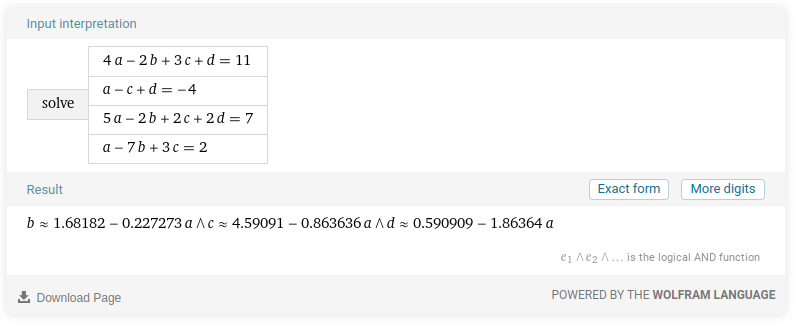
\includegraphics[width=14cm]{images/lineq1.png}
  \caption{Results from WolframAlpha}
  \label{fig:lineq1}
\end{figure}

\subsection{Equation 2}
\begin{lstlisting}[language=Python, style=jupycolors]
A2=np.matrix([[3.0, 7.0,  1.0,  3.0],
             [1.0, -6.0,  6.0,  9.0],
             [4.0,  4.0, -7.0,  1.0],
             [-1.0, 3.0,  8.0,  2.0]])

b2=(np.matrix([37,
               11,
               38,
               -1])).transpose()

\end{lstlisting}
We obtain an infinite number of solutions : \\
\begin{resultbox}
  infinite x4 solutions, taking 0
  $[[10.27759197]$ \\
  $ [ 0.75585284]$ \\
  $ [ 0.87625418]$ \\
  $ [ 0.        ]]$
\end{resultbox}
Verification: we see that if we take $a=0$ we have the same solutions
\begin{figure}[H]
  \centering
  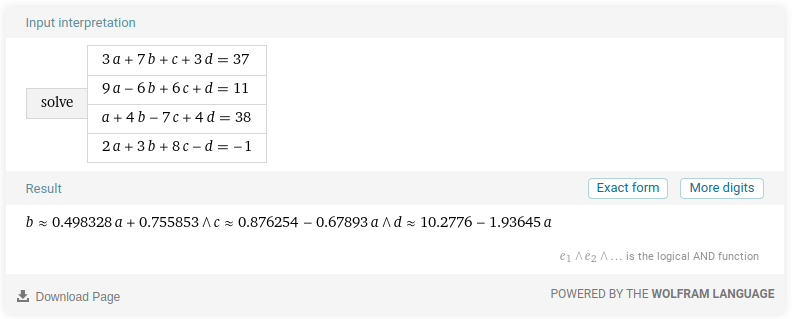
\includegraphics[width=14cm]{images/lineq2.png}
  \caption{Results from WolframAlpha}
  \label{fig:lineq2}
\end{figure}

\subsection{Equation 3}
\begin{lstlisting}[language=Python, style=jupycolors]
A3=np.matrix([[0.0, 1.0,  2.0,  1.0],
             [6.0, -2.0,  3.0,  4.0],
             [0.0,  3.0,  4.0, -3.0],
             [0.0, -4.0,  3.0,  1.0]])

b3=(np.matrix([2,
               -15,
               10,
               -2])).transpose()

\end{lstlisting}
We obtain : \\
\begin{resultbox}
$[[-2.]$\\
$ [ 1.]$\\
$ [ 1.]$\\
$ [-1.]]$
\end{resultbox}
Verification:
\begin{figure}[H]
  \centering
  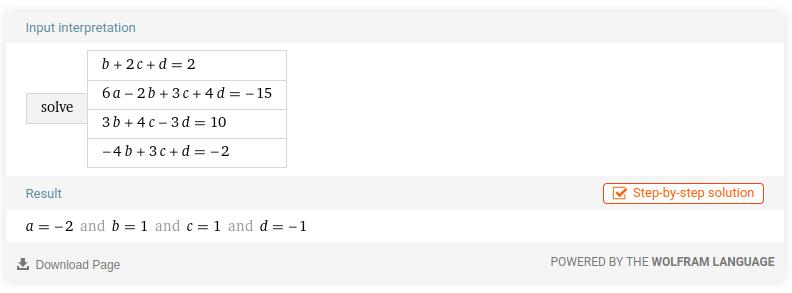
\includegraphics[width=14cm]{images/lineq3.png}
  \caption{Results from WolframAlpha}
  \label{fig:lineq3}
\end{figure}

\subsection{Equation 4}
\begin{lstlisting}[language=Python, style=jupycolors]
A4=np.matrix([[3.0, 7.0,  1.0,  3.0],
             [1.0, -6.0,  6.0,  8.0],
             [4.0,  4.0, -7.0,  1.0],
             [4.0, 16.0,  2.0,  0.0]])

b4=(np.matrix([40,
               19,
               36,
               48])).transpose()

\end{lstlisting}
We obtain : \\
\begin{resultbox}
$[[ 1.]$\\
$ [ 3.]$\\
$ [-2.]$\\
$ [ 6.]]$
\end{resultbox}
Verification:
\begin{figure}[H]
  \centering
  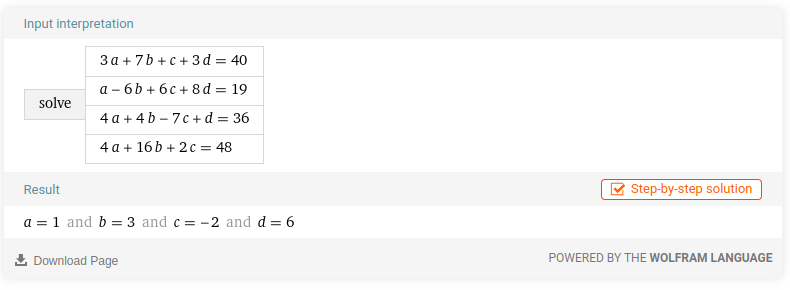
\includegraphics[width=14cm]{images/lineq4.png}
  \caption{Results from WolframAlpha}
  \label{fig:lineq4}
\end{figure}

\subsection{Equation 5}
\begin{lstlisting}[language=Python, style=jupycolors]
A4=np.matrix([[3.0, 7.0,  1.0,  3.0],
             [1.0, -6.0,  6.0,  8.0],
             [4.0,  4.0, -7.0,  1.0],
             [4.0, 16.0,  2.0,  0.0]])

b5=(np.matrix([-4,
               3,
               7,
               2])).transpose()

\end{lstlisting}
We obtain no solution for this system : \\
\begin{resultbox}
    No solution for this system
\end{resultbox}
Verification:
\begin{figure}[H]
  \centering
  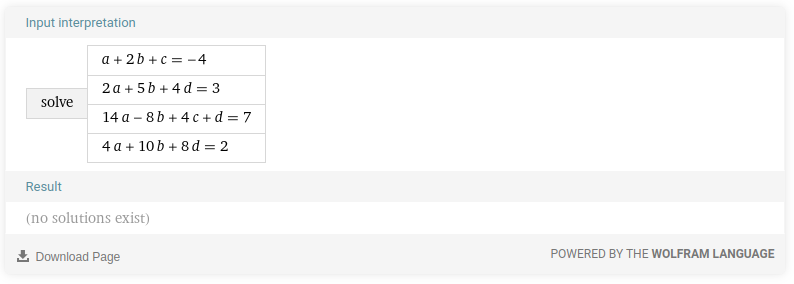
\includegraphics[width=14cm]{images/lineq5.png}
  \caption{Results from WolframAlpha}
  \label{fig:lineq5}
\end{figure}